\chapter{FUNDAMENTAÇÃO TEÓRICA}
\label{cap:fundamentacao}

Este capítulo apresenta os conceitos que sustentam o trabalho. A Seção \ref{sec:plano} discute o plano de ensino e as normas que regem sua elaboração no IFC. As Seções \ref{sec:llm} a \ref{sec:local} tratam dos modelos de linguagem, de suas limitações, das técnicas empregadas para torná-los confiáveis e de sua execução em equipamento local. A Seção \ref{sec:automacao} aborda as ferramentas de automação e infraestrutura, a Seção \ref{sec:humano} discute o papel do avaliador humano e a Seção \ref{sec:metricas} apresenta as métricas de avaliação utilizadas. Por fim, a Seção \ref{sec:relacionados} revisa os trabalhos relacionados.

\section{O plano de ensino e as normas institucionais}
\label{sec:plano}

O planejamento é uma atividade de reflexão e de organização da ação docente, por meio da qual o professor articula os objetivos, os conteúdos, os métodos e a avaliação de forma coerente com a proposta pedagógica da instituição \cite{Libaneo1994}. O plano de ensino é o registro desse planejamento para um componente curricular em um período letivo. Ele serve, ao mesmo tempo, como guia para o docente, como compromisso público com os estudantes e como instrumento de acompanhamento para a gestão do curso.

A LDB estabelece que os docentes devem elaborar e cumprir seu plano de trabalho segundo a proposta pedagógica do estabelecimento e que as instituições de educação superior devem informar aos interessados, antes de cada período letivo, os programas dos cursos e componentes curriculares, seus requisitos e seus critérios de avaliação \cite{Brasil1996}. No IFC, a Organização Didática dos Cursos detalha essas exigências e define os elementos que devem constar no plano de ensino, que é submetido à apreciação da coordenação e do NDE do curso \cite{ifc2022}.

Na prática do IFC, o plano de ensino é registrado no SIGAA e exportado como um documento PDF com estrutura padronizada: identificação do componente e do docente, ementa, metodologia, procedimentos de avaliação, horário de atendimento, objetivos, conteúdo programático, cronograma de aulas, avaliações previstas e referências básicas e complementares. Embora a ordem e os rótulos das seções sejam fixos, o conteúdo de cada seção é texto livre, escrito por docentes diferentes, com estilos, extensões e graus de detalhamento distintos. Essa combinação de estrutura fixa e conteúdo livre é o que motiva a abordagem híbrida adotada neste trabalho: regras determinísticas para o que é estrutural e modelos de linguagem para o que exige interpretação.

\section{Modelos de linguagem}
\label{sec:llm}

Como visto na seção anterior, o plano de ensino tem estrutura fixa, mas o conteúdo de cada seção é texto livre. Verificar se esse conteúdo atende às normas exige uma tecnologia capaz de interpretar linguagem natural, e a que fundamenta este trabalho são os modelos de linguagem. Eles são objeto de estudo do PLN, a área da IA que trata da compreensão e da geração de linguagem humana por computadores \cite{RussellNorvig2021, Jurafsky2025}.

Um modelo de linguagem atribui probabilidades a sequências de palavras e, de forma equivalente, estima a probabilidade da próxima unidade de texto (\textit{token}) dada a sequência anterior \cite{Jurafsky2025}. Os LLMs são modelos de linguagem com bilhões de parâmetros, treinados sobre grandes volumes de texto. Com o aumento de escala, esses modelos passaram a exibir a capacidade de executar tarefas novas apenas a partir de instruções e exemplos fornecidos na entrada, sem ajuste dos pesos, fenômeno conhecido como aprendizado em contexto (\textit{in-context learning}) \cite{Brown2020, Zhao2023}. É essa capacidade que permite usar um mesmo modelo, sem treinamento adicional, para avaliar se uma ementa ou uma metodologia atende a uma regra descrita em linguagem natural.

\subsection{A arquitetura \textit{Transformer}}

A capacidade de executar tarefas a partir de instruções, descrita acima, só se tornou possível com o aumento de escala dos modelos, e esse aumento, por sua vez, foi viabilizado por uma arquitetura específica. Os LLMs atuais são baseados na arquitetura \textit{Transformer}, proposta por \citeonline{Vaswani2017}, que substitui as redes recorrentes por um mecanismo de atenção que, para cada \textit{token}, calcula o quanto cada um dos demais \textit{tokens} da sequência é relevante para sua representação. Na formulação original, a atenção é dada pela Equação \ref{eq:atencao}, em que $Q$, $K$ e $V$ são matrizes de consultas, chaves e valores obtidas por projeções lineares da entrada e $d_k$ é a dimensão das chaves \cite{Vaswani2017}.

\begin{equation}
\label{eq:atencao}
\mathrm{Attention}(Q, K, V) = \mathrm{softmax}\left(\frac{QK^{\top}}{\sqrt{d_k}}\right)V
\end{equation}

Como a atenção relaciona diretamente quaisquer duas posições da sequência, o \textit{Transformer} captura dependências de longa distância e permite paralelizar o treinamento, o que viabilizou o crescimento dos modelos para bilhões de parâmetros. Os modelos generativos, como os da família GPT e o Qwen utilizado neste trabalho, empregam apenas a pilha decodificadora e geram texto de forma autorregressiva, um \textit{token} por vez \cite{Brown2020, Qwen2024}. Durante a geração, as chaves e os valores já calculados são armazenados em um \textit{cache} (\textit{KV cache}) para não serem recomputados, e seu tamanho cresce linearmente com o comprimento do contexto, o que torna o contexto máximo um fator determinante do consumo de memória.

\subsection{Limitações dos LLMs}

A mesma arquitetura que permite aos LLMs gerar texto fluente, um \textit{token} por vez, não garante que esse texto seja correto. Apesar da fluência, os LLMs apresentam limitações relevantes para aplicações de verificação. A principal é a alucinação, definida como a geração de conteúdo sem sentido ou infiel à fonte fornecida \cite{Ji2023}. Em um verificador de documentos, uma alucinação pode se manifestar como a afirmação de que uma seção está ausente quando ela existe, ou o contrário. Outra limitação é a sensibilidade à posição da informação: \citeonline{Liu2024} mostraram que o desempenho de LLMs em contextos longos cai quando a informação relevante está no meio da entrada, o que favorece entradas curtas e bem delimitadas. Os modelos também têm dificuldade com operações exatas, como contagens, e não têm acesso a normas institucionais específicas que não estejam presentes em seus dados de treinamento.

\section{Técnicas para respostas confiáveis}
\label{sec:tecnicas}

As limitações descritas na seção anterior não desaparecem com a simples escolha de um modelo maior. Por isso, foram propostas técnicas que atuam em torno do modelo, sem alterar seus pesos, para tornar suas respostas mais confiáveis. Essas técnicas interferem em três pontos do processo. Na entrada, definem o que o modelo recebe: instruções bem estruturadas e o conhecimento necessário para a tarefa, como fazem a engenharia de \textit{prompt} e a geração aumentada por recuperação. Na saída, restringem o formato da resposta para que ela possa ser processada por software, como faz a geração estruturada. Na verificação, conferem o julgamento do modelo ou o substituem por regras exatas quando a tarefa permite. Como nenhuma delas exige treinar novamente o modelo, todas podem ser aplicadas a um modelo aberto executado localmente. As subseções a seguir descrevem cada técnica e a forma como foi aproveitada neste trabalho.

\subsection{Engenharia de \textit{prompt} e contextualização normativa}

A técnica mais direta atua sobre as instruções fornecidas ao modelo. A engenharia de \textit{prompt} consiste em estruturar as instruções fornecidas ao modelo de forma a obter respostas no formato e com a qualidade desejados. \citeonline{White2023} catalogam padrões de \textit{prompt}, entre eles a definição de uma persona (``você é um avaliador de planos de ensino''), a especificação de um modelo de saída e a imposição de restrições explícitas. No contexto deste trabalho, a estratégia central é a contextualização normativa: as regras de cada critério, derivadas da Organização Didática e das orientações da coordenação, são escritas no próprio \textit{prompt}, junto com o texto de cada seção do plano, de modo que o modelo julgue o documento com base nas regras fornecidas e não em seu conhecimento genérico.

\subsection{Geração aumentada por recuperação}

Na contextualização normativa, o conhecimento que o modelo deve usar é escrito diretamente no \textit{prompt}. Quando esse conhecimento é extenso demais para isso, ele pode ser buscado automaticamente. É o que faz a Geração Aumentada por Recuperação (\textit{Retrieval-Augmented Generation}, RAG), proposta por \citeonline{lewis2020}, combina um modelo gerador com um mecanismo de busca: antes de responder, o sistema recupera de uma base externa, normalmente indexada por vetores de \textit{embeddings}, os trechos mais relevantes para a pergunta e os fornece ao modelo como contexto. A técnica reduz alucinações e permite usar conhecimento atualizado ou específico de uma organização sem retreinar o modelo \cite{lewis2020, Gao2023}.

A RAG é especialmente vantajosa quando a base de conhecimento é grande demais para caber no contexto do modelo. No problema tratado aqui, o conhecimento normativo necessário para avaliar um plano se resume a doze regras curtas, que ocupam poucas centenas de \textit{tokens}. Nesse cenário, incluir todas as regras diretamente no \textit{prompt} produz o mesmo efeito de fundamentação da RAG, com menos componentes e sem o risco de a etapa de recuperação deixar de trazer uma regra relevante. Por isso, o sistema desenvolvido adota a contextualização normativa direta, e a RAG com base vetorial é apontada como evolução para quando o sistema precisar consultar documentos extensos, como o PPC completo (Seção \ref{sec:futuros}).

\subsection{Geração estruturada}

As duas técnicas anteriores atuam sobre a entrada do modelo; a geração estruturada atua sobre sua saída. Para que a resposta de um LLM seja processada por software, ela precisa seguir um formato previsível. Pedir ``responda em JSON'' no \textit{prompt} não garante isso: o modelo pode produzir JSON malformado, omitir campos ou usar valores fora do domínio esperado. A geração guiada (\textit{guided} ou \textit{constrained generation}) resolve o problema restringindo, a cada passo da decodificação, os \textit{tokens} admissíveis àqueles que mantêm a saída válida segundo uma gramática ou expressão regular \cite{Willard2023}. O Ollama implementa essa técnica a partir de um JSON Schema informado no parâmetro \texttt{format} da requisição \cite{OllamaStructured, JSONSchema}. Com isso, campos obrigatórios e enumerações, como os valores OK, INCOMPLETO e AUSENTE, passam a ser garantidos pela decodificação e não apenas solicitados ao modelo.

\subsection{LLMs como avaliadores e combinação com regras determinísticas}

Mesmo com uma entrada bem fundamentada e uma saída em formato válido, resta saber se o julgamento do modelo está correto, o que corresponde ao terceiro ponto de atuação, a verificação. Usar um LLM para julgar a qualidade de um texto é uma prática estudada na literatura. \citeonline{Zheng2023} mostraram que LLMs fortes, quando usados como juízes, alcançam concordância com preferências humanas comparável à concordância entre humanos, embora apresentem vieses, como a preferência por respostas mais longas. \citeonline{Gilardi2023} verificaram que um LLM superou anotadores de plataformas de \textit{crowdsourcing} em tarefas de anotação de texto. Ambos os estudos, contudo, reforçam a necessidade de validar as saídas do modelo contra referências humanas, tema também enfatizado na revisão de \citeonline{Chang2024} sobre avaliação de LLMs.

Uma consequência prática dessas limitações é atribuir a cada técnica o tipo de tarefa em que ela é mais confiável. Verificações exatas e estruturais, como contar referências ou detectar uma seção vazia, são resolvidas de forma determinística por código; julgamentos que exigem interpretação, como decidir se uma metodologia descreve como as aulas serão conduzidas, ficam a cargo do LLM. Essa divisão de trabalho é um dos princípios de projeto do sistema descrito no Capítulo \ref{cap:desenvolvimento}.

\section{Execução local de modelos de linguagem}
\label{sec:local}

As técnicas da seção anterior pressupõem um modelo disponível para receber as requisições, que pode ser acessado por um serviço externo ou executado pela própria instituição. Este trabalho adota a segunda opção. Executar um LLM em equipamento próprio evita custos por requisição e mantém os documentos dentro da instituição, mas impõe restrições de memória. Um modelo de 7 bilhões de parâmetros em precisão de 16 bits ocupa cerca de 14 GB apenas com os pesos, acima da memória de vídeo (VRAM) de GPUs de uso pessoal. A quantização reduz esse consumo ao representar os pesos com menos bits, com perda de qualidade pequena quando bem aplicada \cite{Dettmers2022}. O projeto llama.cpp popularizou o formato GGUF e esquemas de quantização como o Q4\_K\_M, que armazena a maior parte dos pesos com cerca de 4 bits \cite{LlamaCpp}. O Ollama, utilizado neste trabalho, empacota esse motor de inferência e expõe os modelos por meio de uma API HTTP local \cite{OllamaDocs}.

O modelo escolhido foi o Qwen2.5 de 7,6 bilhões de parâmetros, um modelo de pesos abertos, distribuído sob a licença Apache 2.0, com suporte a contexto longo, a múltiplos idiomas, incluindo o português, e ênfase declarada na geração de saídas estruturadas como JSON \cite{Qwen2024}. Na versão quantizada Q4\_K\_M, o modelo ocupa cerca de 4,7 GB, o que permite executá-lo em uma GPU de 6 GB, ainda que com pouca margem para o \textit{KV cache}.

Duas otimizações de inferência foram relevantes neste trabalho. O \textit{FlashAttention} reorganiza o cálculo da atenção para reduzir os acessos à memória da GPU, tornando-o mais rápido e econômico sem alterar o resultado \cite{Dao2022}. A quantização do \textit{KV cache} para 8 bits reduz a memória ocupada pelo contexto, permitindo que uma fração maior do modelo permaneça na GPU. O efeito combinado dessas configurações sobre o desempenho do sistema é medido no Capítulo \ref{cap:resultados}.

\section{Automação de fluxos e infraestrutura}
\label{sec:automacao}

O modelo de linguagem, por si só, não forma um sistema: é preciso obter os documentos, extrair seu texto, enviá-lo ao modelo, registrar as respostas e executar tudo isso de forma reprodutível. Esta seção apresenta as ferramentas usadas para essa orquestração. O n8n é uma plataforma de automação de fluxos de trabalho de código-fonte disponível, na qual um fluxo (\textit{workflow}) é composto visualmente por nós conectados. Cada nó executa uma operação, como acionar o fluxo em um horário, ler arquivos de um serviço de armazenamento, fazer uma requisição HTTP ou executar um trecho de código JavaScript, e entrega uma lista de itens ao nó seguinte \cite{n8nDocs}. A plataforma oferece integrações prontas com serviços como Google Drive e Google Sheets, autenticadas por OAuth 2.0, e permite expor fluxos como \textit{webhooks}, isto é, como endereços HTTP que executam o fluxo ao serem acessados. Essas características permitem construir um \textit{pipeline} completo de processamento de documentos sem desenvolver uma aplicação do zero, e o histórico de execuções mantido pela plataforma facilita a depuração e a auditoria.

O Docker permite empacotar uma aplicação e suas dependências em contêineres isolados e reprodutíveis, que se comportam da mesma forma em qualquer máquina com o Docker instalado \cite{Merkel2014}. O Docker Compose descreve, em um único arquivo, os contêineres de um sistema, suas redes, volumes e recursos, como o acesso à GPU. A operação de sistemas com componentes de aprendizado de máquina em produção exige ainda práticas de MLOps, como versionamento de configurações, monitoramento das saídas e reprodutibilidade das execuções \cite{Kreuzberger2023}, que orientaram a forma como o sistema registra cada validação.

Por fim, a extração de texto de documentos PDF é feita pelo n8n com base na biblioteca PDF.js \cite{PDFjs}, que reconstrói o texto a partir dos objetos gráficos do documento. Como o PDF não armazena a estrutura lógica do texto, o resultado preserva as quebras de linha da diagramação, intercala cabeçalhos e rodapés de página com o conteúdo e não distingue as colunas de tabelas, características que influenciam o projeto da etapa de segmentação.

\section{IA centrada no ser humano}
\label{sec:humano}

As seções anteriores trataram dos componentes técnicos do sistema; falta definir o papel das pessoas que usam seus resultados, já que, como visto na Seção \ref{sec:llm}, o modelo pode errar. \citeonline{Shneiderman2022} defende que sistemas de IA devem ampliar a capacidade humana, combinando altos níveis de automação com altos níveis de controle humano, em vez de substituir o julgamento das pessoas. As diretrizes de interação humano-IA de \citeonline{Amershi2019} recomendam, entre outros pontos, deixar claro o que o sistema faz e com que qualidade, explicar por que ele tomou cada decisão e facilitar a correção quando ele erra. No campo educacional, o relatório do \citeonline{USDeptEd2023} recomenda manter o ser humano no circuito decisório (\textit{humans in the loop}) em qualquer uso de IA que afete estudantes e educadores.

Esses princípios orientaram três características do sistema: ele não aprova nem reprova planos de forma definitiva, apenas sinaliza possíveis não conformidades; cada apontamento vem acompanhado de uma justificativa; e o painel oferece acesso direto ao PDF original para que o avaliador confirme ou descarte o apontamento.

\section{Métricas de avaliação}
\label{sec:metricas}

Manter o avaliador humano no circuito não dispensa medir a qualidade dos apontamentos do sistema, pois é dela que depende a confiança desse avaliador. Como o sistema atribui a cada critério uma classe, sua qualidade pode ser medida com as métricas usuais de classificação. Para avaliar um classificador, compara-se sua saída com uma referência considerada correta (\textit{ground truth}). Neste trabalho, a tarefa é tratada como classificação binária por critério, em que a classe positiva é a não conformidade: o sistema acerta quando aponta um problema que de fato existe. As quatro situações possíveis compõem a matriz de confusão: verdadeiro positivo (VP), quando o sistema aponta uma não conformidade real; falso positivo (FP), quando aponta um problema inexistente; falso negativo (FN), quando deixa de apontar um problema real; e verdadeiro negativo (VN), quando considera conforme um item conforme \cite{Sokolova2009}. A partir delas são definidas as métricas das Equações \ref{eq:acuracia} a \ref{eq:f1} \cite{Sokolova2009}.

\begin{equation}
\label{eq:acuracia}
\mathrm{Acur\acute{a}cia} = \frac{VP + VN}{VP + FP + FN + VN}
\end{equation}

\begin{equation}
\label{eq:precisao}
\mathrm{Precis\tilde{a}o} = \frac{VP}{VP + FP}
\end{equation}

\begin{equation}
\label{eq:recall}
\mathrm{Recall} = \frac{VP}{VP + FN}
\end{equation}

\begin{equation}
\label{eq:f1}
F_1 = 2 \cdot \frac{\mathrm{Precis\tilde{a}o} \cdot \mathrm{Recall}}{\mathrm{Precis\tilde{a}o} + \mathrm{Recall}}
\end{equation}

A precisão indica, entre os itens apontados como problemáticos, quantos realmente o eram; o \textit{recall}, ou sensibilidade, indica quantos dos problemas existentes foram encontrados. Em uma ferramenta de triagem, o \textit{recall} tende a ser mais importante, pois um falso negativo deixa passar um plano irregular, enquanto um falso positivo apenas gera uma revisão humana desnecessária. O $F_1$ é a média harmônica entre as duas.

Quando a classe positiva é rara, a acurácia pode ser alta mesmo para um classificador trivial. O coeficiente Kappa de Cohen corrige esse efeito ao descontar a concordância esperada ao acaso \cite{Cohen1960}, conforme a Equação \ref{eq:kappa}, em que $p_o$ é a proporção de concordância observada e $p_e$ é a proporção esperada ao acaso, calculada a partir das frequências marginais de cada classe.

\begin{equation}
\label{eq:kappa}
\kappa = \frac{p_o - p_e}{1 - p_e}
\end{equation}

O Kappa vale 1 para concordância perfeita e 0 para concordância equivalente ao acaso. \citeonline{Landis1977} propuseram a interpretação mais difundida para seus valores: abaixo de 0 indica concordância pobre; de 0,00 a 0,20, leve; de 0,21 a 0,40, razoável; de 0,41 a 0,60, moderada; de 0,61 a 0,80, substancial; e de 0,81 a 1,00, quase perfeita.

\section{Trabalhos relacionados}
\label{sec:relacionados}

Definidos os conceitos técnicos e as métricas, esta seção situa o trabalho em relação à produção acadêmica sobre IA na educação, com atenção especial ao seu uso em processos administrativos. O emprego de IA na educação tem crescido de forma acentuada. A análise bibliométrica de \citeonline{Metli2023}, que examinou 6.498 artigos indexados na \textit{Web of Science} entre 1984 e 2022, identificou crescimento anual de 22,68\% nas publicações sobre IA e educação. Como mostra a Figura \ref{fig:publicacoes_ia}, a produção anual permaneceu abaixo de 100 artigos até 2014 e acelerou a partir de 2019, chegando a 2.361 artigos em 2022.

\begin{figure}[H]
\centering
\caption{Artigos publicados por ano sobre IA e educação (2006--2022)}
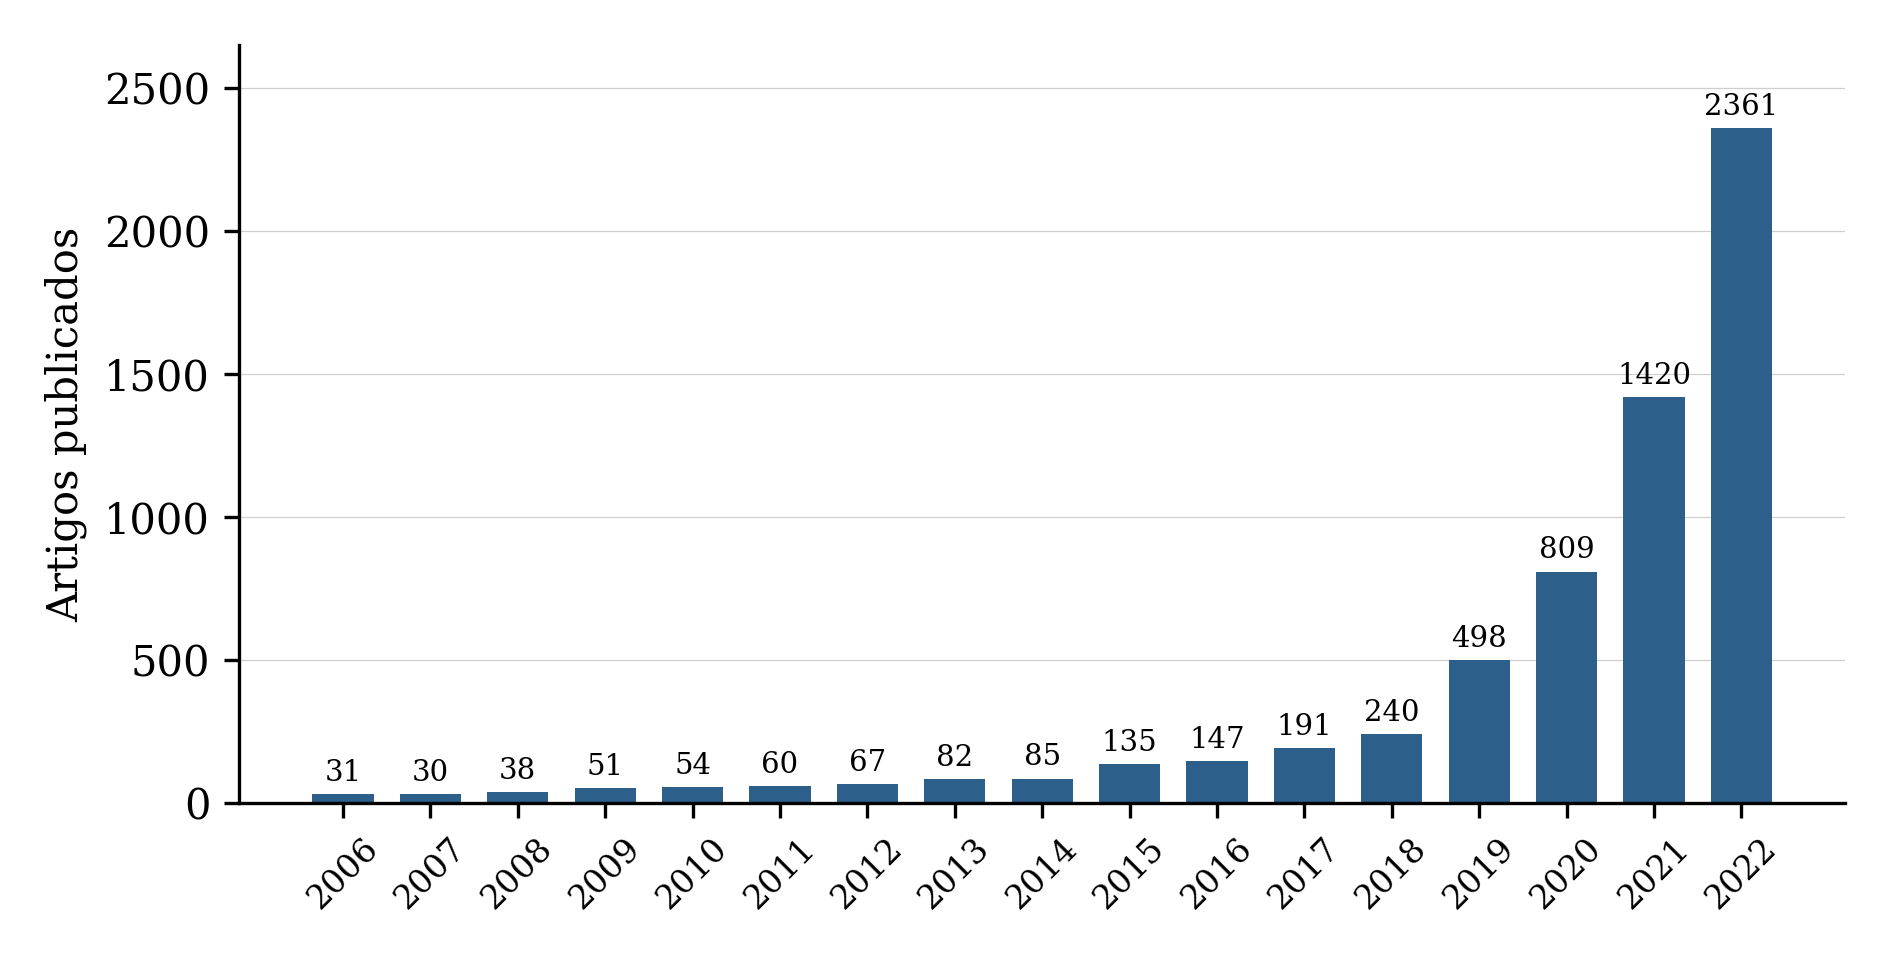
\includegraphics[width=0.85\textwidth]{images/publicacoes_ia_metli.png}
\label{fig:publicacoes_ia}
\legend{Fonte: Elaborado pelo autor com dados de \citeonline{Metli2023}.}
\end{figure}

Dentro desse volume crescente de publicações, foram selecionados sete trabalhos que tratam do uso de IA no ensino e na gestão educacional, descritos a seguir. O primeiro é a revisão sistemática de \citeonline{Tan2025}, que analisou 95 publicações de 2015 a 2024 sobre IA no ensino e no desenvolvimento profissional docente e identificou aplicações em planejamento de aulas, avaliação automatizada, \textit{feedback} individualizado e otimização de tarefas administrativas. Os autores apontam, porém, a escassez de estudos sobre processos administrativos de instituições de ensino superior, lacuna na qual este trabalho se insere.

O trabalho de \citeonline{Kasneci2023}, um ensaio crítico, discute as oportunidades e os desafios dos LLMs na educação. Entre os riscos, os autores destacam a confiança excessiva nas respostas do modelo e a necessidade de supervisão humana e de transparência, preocupações que orientaram a decisão de manter o avaliador humano como responsável pela decisão final no sistema aqui desenvolvido.

Com foco na gestão, \citeonline{Sposato2025} propõe uma taxonomia das aplicações de IA na liderança e na administração de instituições de ensino. A automação de análises documentais aparece nessa taxonomia entre os usos administrativos, mas de forma conceitual, sem a implementação de um sistema.

Já \citeonline{Hoare2025} relatam a experiência do Departamento de Educação de Nova Gales do Sul, na Austrália, que desenvolveu uma ferramenta própria de IA generativa, o NSWEduChat, testada em 50 escolas a partir de 2024 para apoiar práticas de ensino baseadas em evidências. Entre os mais de 100 professores participantes da formação associada, 95\% afirmaram que a ferramenta economizaria tempo. O estudo destaca que a contextualização das respostas com materiais e diretrizes institucionais foi decisiva para a confiança dos docentes, o que apoia a estratégia de fundamentar a avaliação nas normas do IFC.

No contexto brasileiro, \citeonline{Santos2025} analisam a adoção de plataformas digitais e de IA na gestão de redes públicas de ensino e alertam que a centralização dessas plataformas pode restringir a autonomia dos atores escolares, concluindo que uma adoção responsável exige transparência no uso dos dados e infraestrutura adequada.

Mais próximo do contexto deste trabalho, \citeonline{Vieira2025} realizaram uma revisão integrativa sobre IA nos Institutos Federais. Os autores constataram pouca produção acadêmica sobre o tema e identificaram a IA como apoio administrativo como a forma de incorporação menos explorada na rede federal.

Por fim, \citeonline{VieiraFilho2024} aplica técnicas de PLN em Python à recomendação de conteúdo educacional em português. Embora não trate de processos administrativos, o trabalho demonstra a viabilidade dessas técnicas sobre textos acadêmicos no idioma, condição necessária para a abordagem adotada aqui.

A Tabela \ref{tab:relacionados} sintetiza a comparação entre os sete trabalhos descritos nesta seção e a proposta deste trabalho. A análise bibliométrica de \citeonline{Metli2023} não foi incluída na comparação por tratar do volume de publicações sobre o tema, e não de uma aplicação específica de IA.

\begin{table}[H]
\centering
\caption{Comparação entre os trabalhos relacionados e este trabalho}
\label{tab:relacionados}
\footnotesize
\begin{tabular}{@{}L{3.1cm}L{3.4cm}L{2.6cm}L{2.2cm}L{2.4cm}@{}}
\toprule
\rowcolor[HTML]{EFEFEF}
\textbf{Trabalho} & \textbf{Foco} & \textbf{Tipo de estudo} & \textbf{Contexto} & \textbf{Processo administrativo?} \\ \midrule
\citeonline{Tan2025} & IA no ensino e na formação docente & Revisão sistemática & Internacional & Apontado como lacuna \\
\citeonline{Kasneci2023} & Oportunidades e riscos de LLMs na educação & Ensaio crítico & Internacional & Não \\
\citeonline{Sposato2025} & IA na gestão educacional & Taxonomia & Internacional & Sim, conceitual \\
\citeonline{Hoare2025} & Ferramenta institucional de IA generativa & Relato de implantação & Austrália, educação básica & Não \\
\citeonline{Santos2025} & Plataformas e IA na gestão pública & Análise documental & Brasil, redes públicas & Sim, conceitual \\
\citeonline{Vieira2025} & IA nos Institutos Federais & Revisão integrativa & Brasil, rede federal & Apontado como lacuna \\
\citeonline{VieiraFilho2024} & PLN para recomendação de conteúdo & Desenvolvimento de sistema & Brasil, ensino superior & Não \\
\textbf{Este trabalho} & \textbf{Validação de planos de ensino} & \textbf{Sistema e estudo de caso} & \textbf{IFC Videira} & \textbf{Sim, implementado e avaliado} \\ \bottomrule
\end{tabular}
\legend{Fonte: Elaborado pelo autor (2026).}
\end{table}

Os trabalhos revisados confirmam o interesse crescente pela IA na educação, mas tratam a gestão administrativa de forma conceitual ou a apontam como lacuna. Nenhum deles implementa e avalia um sistema para a verificação de planos de ensino frente a normas institucionais. Este trabalho busca contribuir para preencher essa lacuna com uma solução implementada, de baixo custo, executada localmente e avaliada sobre documentos reais de um Instituto Federal da região Sul.
